\chapter{Preface}

\section{Introduction}
This document tries to demonstrate the \gnutls{} library API, the
protocols and the technology involved. I believe that a basic
understanding of the underlying protocols is important, before
using \tls{}. This is because security and cryptographic
protocols are involved, which require the application programmer
to make correct use of these protocols, or no security is
offered. Although this document tries to be self contained basic 
network programming and PKI knowlegde is assumed in most of this document. 
I suggest \cite{GUTPKI} for an introduction to PKI.

\chapter{The Library}

\section{Description}
\par
In brief \gnutls{} can be described as a library which offers
an API to access secure communication protocols. These protocols provide
privacy over insecure lines, and were designed to prevent 
eavesdropping, tampering, or message forgery.

\par
Technically \gnutls{} is a portable ANSI {\bf C} based library which implements the 
\tlsI{}\footnote{See section \ref{sec:tlsintro} on page \pageref{sec:tlsintro} for
a more detailed description of the protocols.} and \sslIII{} protocols. 
The library is available under the GNU Lesser GPL license\footnote{A copy of the license is included
in the distribution}.
Important features of the \gnutls{} library include:

\begin{itemize}
\item Thread safety
\item Support for both \tlsI{} and \sslIII{} protocols.
\item Support for both {\bf X.509} and {\bf OpenPGP} certificates.
\item Support for handling and verification of certificates.
\item Support for {\bf SRP} for \tls{} authentication.
\item Support for \tls{} {\bf Extension mechanism}.
\item Support for \tls{} {\bf Compression Methods}.
\end{itemize}

Additionaly \gnutls{} provides a limited emulation API for the widely used
OpenSSL\footnote{\htmladdnormallink{http://www.openssl.org/}{http://www.openssl.org/}} 
library, to ease integration with existing applications.

\par 
\gnutls{} consists of three
independent parts, namely the ``TLS protocol part'', the ``Certificate part'', and 
the ``Crypto backend'' part.
The `TLS protocol part' is the actual protocol implementation, and is entirely
implemented within the \gnutls{} library.
The `Certificate part' consists of the certificate parsing, and verification
functions which is partially implemented in the \gnutls{} library. The
Libtasn1\footnote{\htmladdnormallink{ftp://ftp.gnupg.org/gcrypt/alpha/gnutls/libtasn1/}{ftp://ftp.gnupg.org/gcrypt/alpha/gnutls/libtasn1/}}
a library which offers ASN.1 parsing capabilities, is used for the
X.509 certificate parsing functions, and
Opencdk\footnote{\htmladdnormallink{ftp://ftp.gnupg.org/gcrypt/alpha/gnutls/opencdk/}{ftp://ftp.gnupg.org/gcrypt/alpha/gnutls/opencdk/}}
is used for the OpenPGP key support in \gnutls{}.
The `Crypto backend' is provided by the 
libgcrypt\footnote{\htmladdnormallink{ftp://ftp.gnupg.org/gcrypt/alpha/libgcrypt/}{ftp://ftp.gnupg.org/gcrypt/alpha/libgcrypt/}}
library.
\par
In order to ease integration in embedded systems, parts of the \gnutls{} library 
can be disabled at compile time. That way a small library, with the required features,
can be generated.

\par
See \htmladdnormallink{http://www.gnutls.org/}{http://www.gnutls.org/}
and \htmladdnormallink{http://www.gnu.org/software/gnutls/}{http://www.gnu.org/software/gnutls/} 
for updated versions of the \gnutls{} software and this document.


\section{General Idea}
% explain how it works
A brief description of how \gnutls{} works internally is shown at
the figure \ref{fig:internals}. This section may be easier to understand
after having seen the examples on page \pageref{examples}.

\begin{figure}[htp]
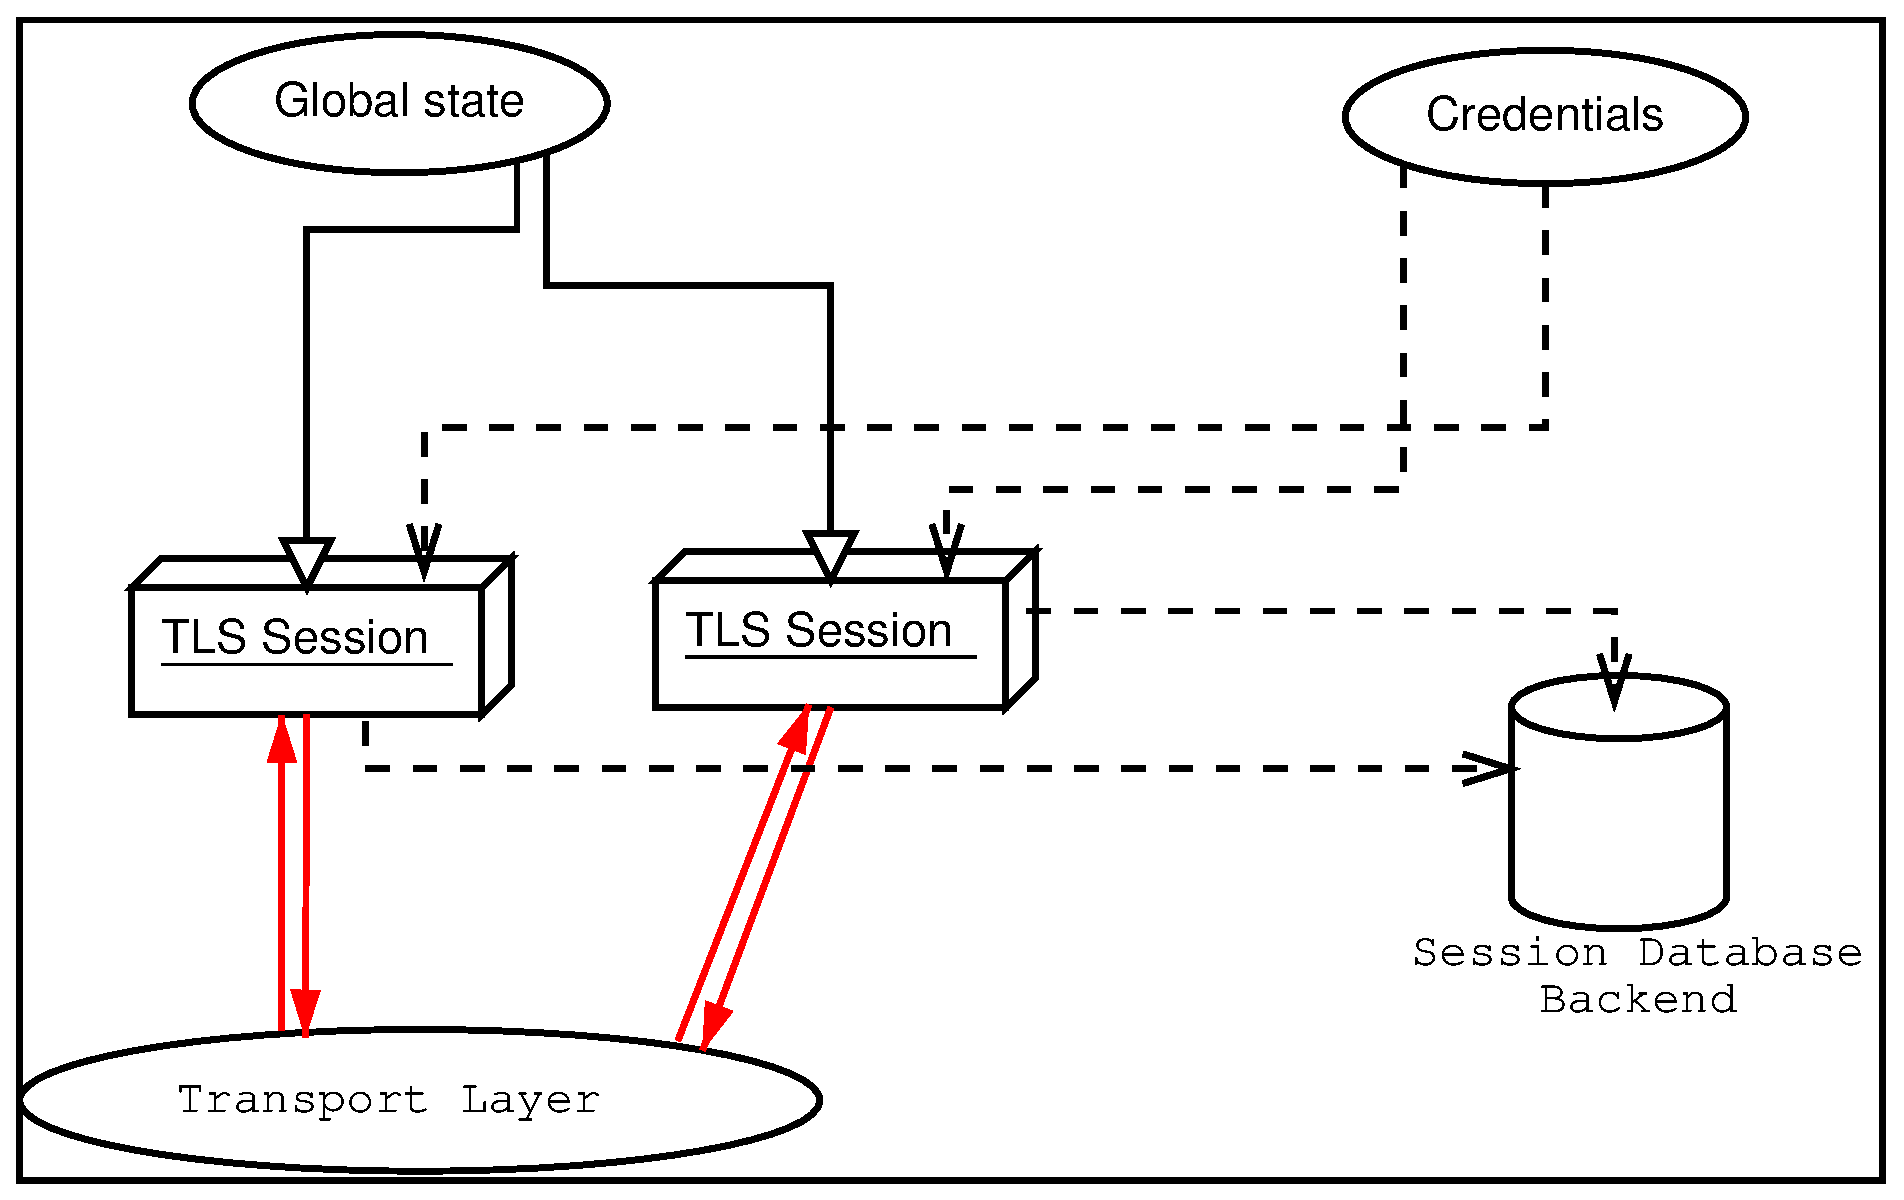
\includegraphics[height=8cm,width=12cm]{internals}
\label{fig:internals}
\end{figure}

\par
As shown in the figure, there is a read-only global state that
is initialized once by the global initialization function.
This global structure, among others, contains the memory allocation
functions used, and some structures needed for the ASN.1 parser.
This structure is never modified by any \gnutls{} function, except
for the deinitialization function which frees all memory allocated in
the global structure and is called after the program has permanently finished 
using \gnutls{}.

\par
The credentials structure is used by some authentication methods,
such as certificate authentication\footnote{see section \ref{certificate} on page \pageref{certificate}}.
A credentials structure may contain certificates, private keys, temporary parameters 
for diffie hellman or RSA key exchange, and other stuff that may be shared
between several TLS sessions. 

This structure should be initialized using the appropriate initialization
functions. For example an application which uses certificate authentication
would probably initialize the credentials, using the appropriate functions,
and put its trusted certificates in this structure. The next step is to
associate the credentials structure with each \tls{} session.

\par A \gnutls{} session contains all the required stuff for a
session to handle one secure connection. This session calls directly
to the transport layer functions, in order to communicate with the peer.
Every session has a unique session ID shared with the peer.

\par
Since TLS sessions can be resumed, servers would probably need a database
backend to hold the session's parameters. Every \gnutls{} session after
a successful handshake calls the appropriate backend function\footnote{see section \ref{resume}
on \pageref{resume} for information on initialization} to store the
newly negotiated session. The session database is examined by the server
just after having received the client hello\footnote{The first message
in a \tls{} handshake}, and if the session ID sent by the client,
matches a stored session, the stored session will be retrieved, and the
new session will be a resumed one, and will share the same session ID
with the previous one.

\section{Error Handling}
\par
In \gnutls most functions return an integer type as a result.
In almost all cases a zero or a positive number means success, and
a negative number indicates failure, or a situation that some
action has to be taken. Thus negative error codes may be fatal
or not. 
\par 
Fatal errors terminate the connection immediately and
further sends ard receives will be disallowed. An example of
a fatal error code is GNUTLS\_E\_MAC\_FAILED. Non-fatal errors
may warn about something (ie a warning alert was received), or
indicate the some action has to be taken. This is the case with
the error code GNUTLS\_E\_REHANDSHAKE returned by 
\hyperref{gnutls\_record\_recv()}{gnutls\_record\_recv() (see Section }{)}{gnutls_record_recv}.
This error code indicates that the server requests a rehandshake. The client
may ignore this request, or may reply with an alert.
You can test if an error code is a fatal one by using the
\hyperref{gnutls\_error\_is\_fatal()}{gnutls\_error\_is\_fatal() (see Section }{)}{gnutls_error_is_fatal}.
\par
If any non fatal errors, that require reaction, are to be returned by a
function, these error codes will be documented
in the function's reference.



\section{Memory handling}

\gnutls{} internally handles heap allocated objects differently, depending
on the sensitivity of the data they contain. However for performance
reasons, the default memory functions do not overwrite sensitive data from
memory, nor protect such objects from being written to the swap. 
In order to change the default behavior the
\printfunc{gnutls_global_set_mem_functions}{gnutls\_global\_set\_mem\_functions}
function is available which can be used to set other memory 
handlers than the defaults. 
\par
The \emph{libgcrypt} library on which \gnutls{} depends, has such secure
memory allocation functions available. These should be used in cases
where even the system's swap memory is not considered secure. See
the documentation of \emph{libgcrypt} for more information.




\section{Callback functions}
\index{Callback functions}

There are several cases where \gnutls{} may need some out of band input from
your program. This is now implemented using some callback functions,
which your program is expected to register.

An example of this type of functions are the push and pull callbacks
which are used to specify the functions that will retrieve and send
data to the transport layer.
\begin{itemize}
\item \printfunc{gnutls_transport_set_push_function}{gnutls\_transport\_set\_push\_function}
\item \printfunc{gnutls_transport_set_pull_function}{gnutls\_transport\_set\_pull\_function}
\end{itemize}

Other callback functions such as the one set by
\printfunc{gnutls_srp_set_server_credentials_function}{gnutls\_srp\_set\_server\_credentials\_function},
may require more complicated input, including data to be allocated.
These callbacks should allocate and free memory using the functions shown below.
\begin{itemize}
\item \printfunc{gnutls_malloc}{gnutls\_malloc}
\item \printfunc{gnutls_free}{gnutls\_free}
\end{itemize}

